\chapter{序論}

\section{はじめに}
1953年James WatsonとFrancis Crickは、遺伝情報の実体が4種類の塩基による相補的塩基対を形成し、二重らせん構造を持つことを鮮やかに示した。Clickはその5年後、"Ideas for protein synthesis"において、遺伝情報はDNA-RNA-タンパク質へと一方向性を持って伝達されるという分子生物学における中心原理をセントラルドグマとして提唱した。1960年代から70年代には、Maurice WilkinsやSydney Brennerなど多くの研究者によって、コドンの発見と遺伝暗号表が解読され、塩基配列がタンパク質を表現する基本原則が明らかにされてきた。このように、黎明期における分子生物学は、当時の物理学者が多く参入した経緯も相まって、分子のことばで生命の持つ普遍的性質の理解を標榜する学問として誕生した。
\par
今日までの分子生物学研究の急速な発展は、普遍的だと考えられてきた数々の性質や分子機序からの逸脱や例外をも同時に明らかにしてきた。1970年、Howard TeminおよびDavid Baltimoreは一本鎖RNAをテンプレートとして、相補的なDNAを合成する逆転写酵素を発見した。この発見は、セントラルドグマから逸脱し、RNAからDNAへも遺伝情報は伝達しうることを示した画期的な発見であった。その後も、真核生物における遺伝子はスプライシング機構によってイントロンが切り出された複数のエクソンから構成されること、転写直後の新生RNAは3'末端にポリアデニル化、5'末端にはキャップ構造が付加されて成熟すること、コドンが異なるアミノ酸をコードする例外が発見されてきた。こうった発見からセントラルドグマの概念そのものが拡張されてきた。このことは本質的には生命が多様性を担保する存在であることに他ならない。生命が持つ普遍的な性質の理解を目指した分子生物学において、逸脱や例外を対象することが逆説的には、生命を理解することに接続される重要なアプローチになるのだと私は考える。
\par
転写はゲノム上にコードされた遺伝情報をRNAへ正確にコピーする機構を指す。転写は核内で起こる生化学反応であり、RNAポリメラーゼよって触媒される。転写されたpre-mRNAはスプライシング、ポリアデニル化と5'キャップ付加を受けて成熟した後に、核膜孔を通して細胞質へ輸送される、というのが転写機構の大まかな素描である。ヒトゲノムの解読前、遺伝子数はおよそ10万個だと見積もられていたが、解読の完了によって2.5万個程度に大きく下方修正され、直感的な生命の複雑性とゲノムサイズや遺伝子数には相関関係が見られないことは今日に繰り返すまでもない。
\par
真核生物の見せる多様性で複雑なシステムの多くは、転写後および翻訳後の転写物やタンパク質への修飾によって大部分が担保されていることが明らかとなってきた。細胞の内外の情報伝達の多くは、キナーゼによるタンパク質のカスケード的なリン酸化が引き金となり、転写因子が特定の遺伝子発現を制御する。このように、真核生物においては有限個の遺伝子にその多様性を規定されながらも、セントラルドグマに則った転写機構へ逸脱や修飾を加える転写後修飾および翻訳後修飾という機序による多様かつ複雑な制御の重要性が強調されている。
\par
本研究は、セントラルドグマからの逸脱したRNA editingという転写後修飾に注目した研究である。RNA editingはDNAにコードされた遺伝情報がRNAへ転写された後に修飾を受け、別の塩基に置換される現象を指す。本論では、まず今日までに明らかにされたRNA editingの生物学的な機能、制御機構について解説した後に、高出力かつ定量的なオミックスデータを用いたRNA editing研究の現状とその問題をを提起する。第2章では、計算機を持いたRNA editingサイトの網羅的な検出手法の性能評価を行った。第3章では既存の手法の比較からの知見を活かし、高精度かつ高速なRNA editingサイトの検出手法を新規に開発した。第4章では、開発した検出ソフトウェアをヨコヅナクマムシに適用し、極限環境耐性とRNA editingの関係性についての情報学的解析を行った。

\section{真核生物におけるADARの作用機序}
\subsection{ADARによるA-to-I editing}
\par
本研究は転写後修飾のとして最もよく知られるRNA editingと呼ばれる現象に着目している。RNA editingは転写物への一塩基修飾を指し、鞭毛虫のミトコンドリアRNAから初めて発見された。真核生物では、アデニン(A)からイノシン(I)へ修飾されるA-to-I editingの他に、シトシン(C)からチミン(T)への修飾がこれまで報告されている。植物においてはT-to-C editing、ヒトやマウス、ショウジョウバエなど高等真核生物においてはA-to-I editingが優勢を占めることが多くの研究から明らかになっている。
\par
しかしながら、アミノ酸配列の変化を伴うA-to-I editingの報告例は非コード領域におけるeditingに対して著しく少なく、非翻訳領域 (Untranslated regions, UTRs)やAlu配列といったイントロン内のレトロトランスポゾン領域におけるA-to-I editingが優勢を占めていることが明らかになっている。加えて、miRNAやRNAi経路とのクロストークを介したグローバルな遺伝子発現制御との関係性などが指摘されていることから、真核生物におけるA-to-I editingを理解するためには、non-coding RNAにおけるA-to-I editingを研究することが極めて重要であると言える。
から、non-coding RNAへのeditingを介した遺伝子発現制御にA-to-I editingが介在し、制御しうる可能性が徐々に明らかになりつつある。
すなわち、真核生物におけるRNA editingの理解には、従来想定されてきたようなアミノ酸置換を伴ったコード領域内へのeditingのみならず、非コード領域におけるeditingを研究し、その意味を理解することの重要性を示している。本論はこの視点に立脚し、RNA editing研究に関する最新の研究成果を出来うる限り盛り込むようなレビューに努めると同時に、今後のediting研究の進むであろう一つの方向性を示すことができればと考える。

\subsection{ADARの作用機序}
ADAR (adenosine deaminase acting on RNA)は、二本鎖RNA結合タンパクの一種として知られ、相補鎖を形成した二本鎖RNAと選択的に結合し、イノシンへの置換を触媒する (A-to-I editing)。イノシンへと置換された塩基は、転写機構においてグアノシンとして認識される。Guanosine receptor-2 (GluR2)やSerotonin receptor-2C (5-HTR)など位置特異的なA-to-I editingにおいては、隣接するエクソン-イントロン境界における相補的な配列、ECS (Editing-site complamentary sequence)およびその二次構造の形成が不可欠であることが知られている。
\par
加えて、Glutamine receptor (GluR)においては、editingサイト毎にADAR1またはADAR2のどちらか一方に選択的にeditingされることが知られており、位置毎におけるADARの選択性は、ADARの持つdsRBDの数とドメイン間の配列長の相違によるADARと二本鎖RNAとの相互作用が異なることに起因するとの報告がある。

以下にADARによるRNA editingの概略を示す。
\begin{figure}[htbp]
	\begin{center}
		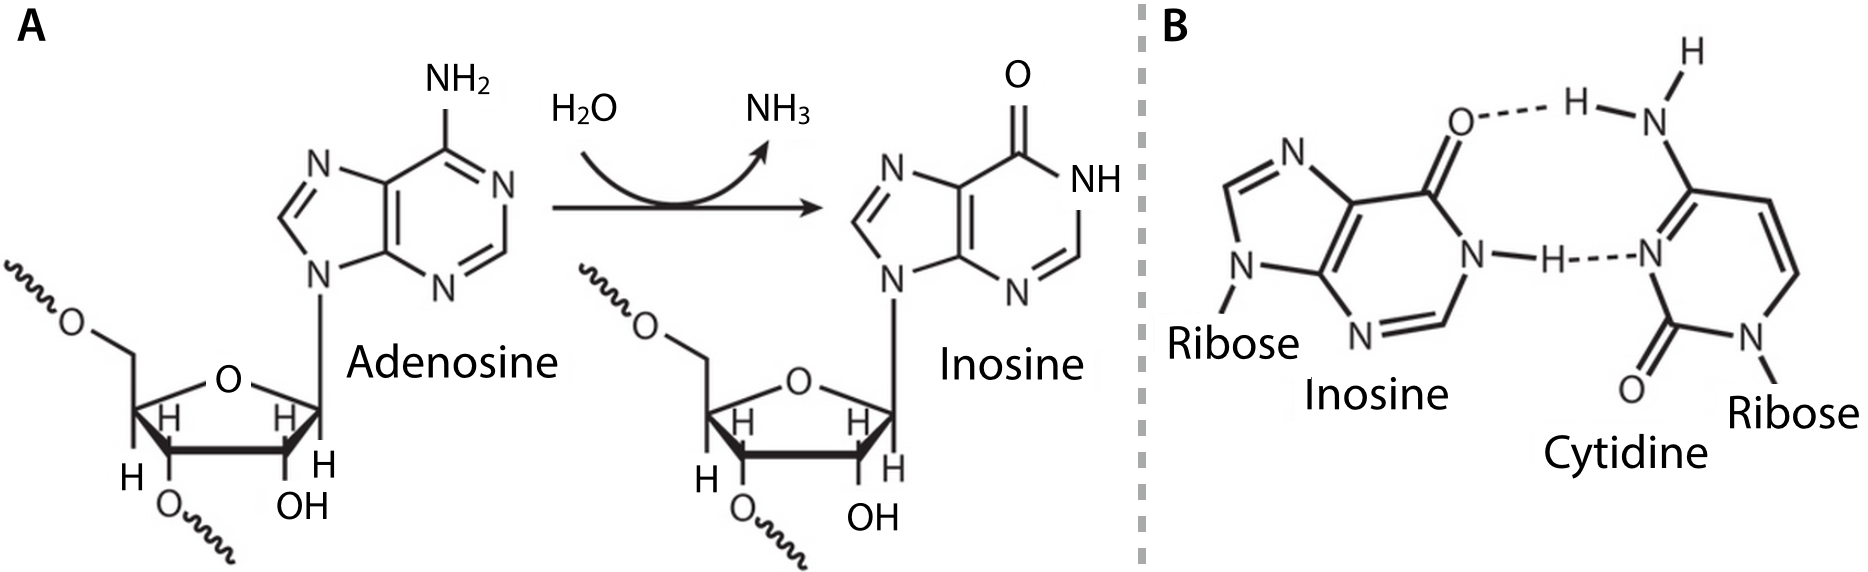
\includegraphics[width=14cm]{Adenosine-inosine.png}
	\end{center}
	\caption{ADARの生化学的な作用機序}
	\begin{flushleft}
		\normalsize{ADARによるアデノシンからイノシンへの化学修飾が触媒される様子を示す。アデノシン塩基はADARによる脱アミノ化反応によってイノシン塩基へと修飾される。}
	\end{flushleft}
	\label{fig:Chemical_reaction}
\end{figure}

\begin{figure}[htbp]
	\begin{center}
		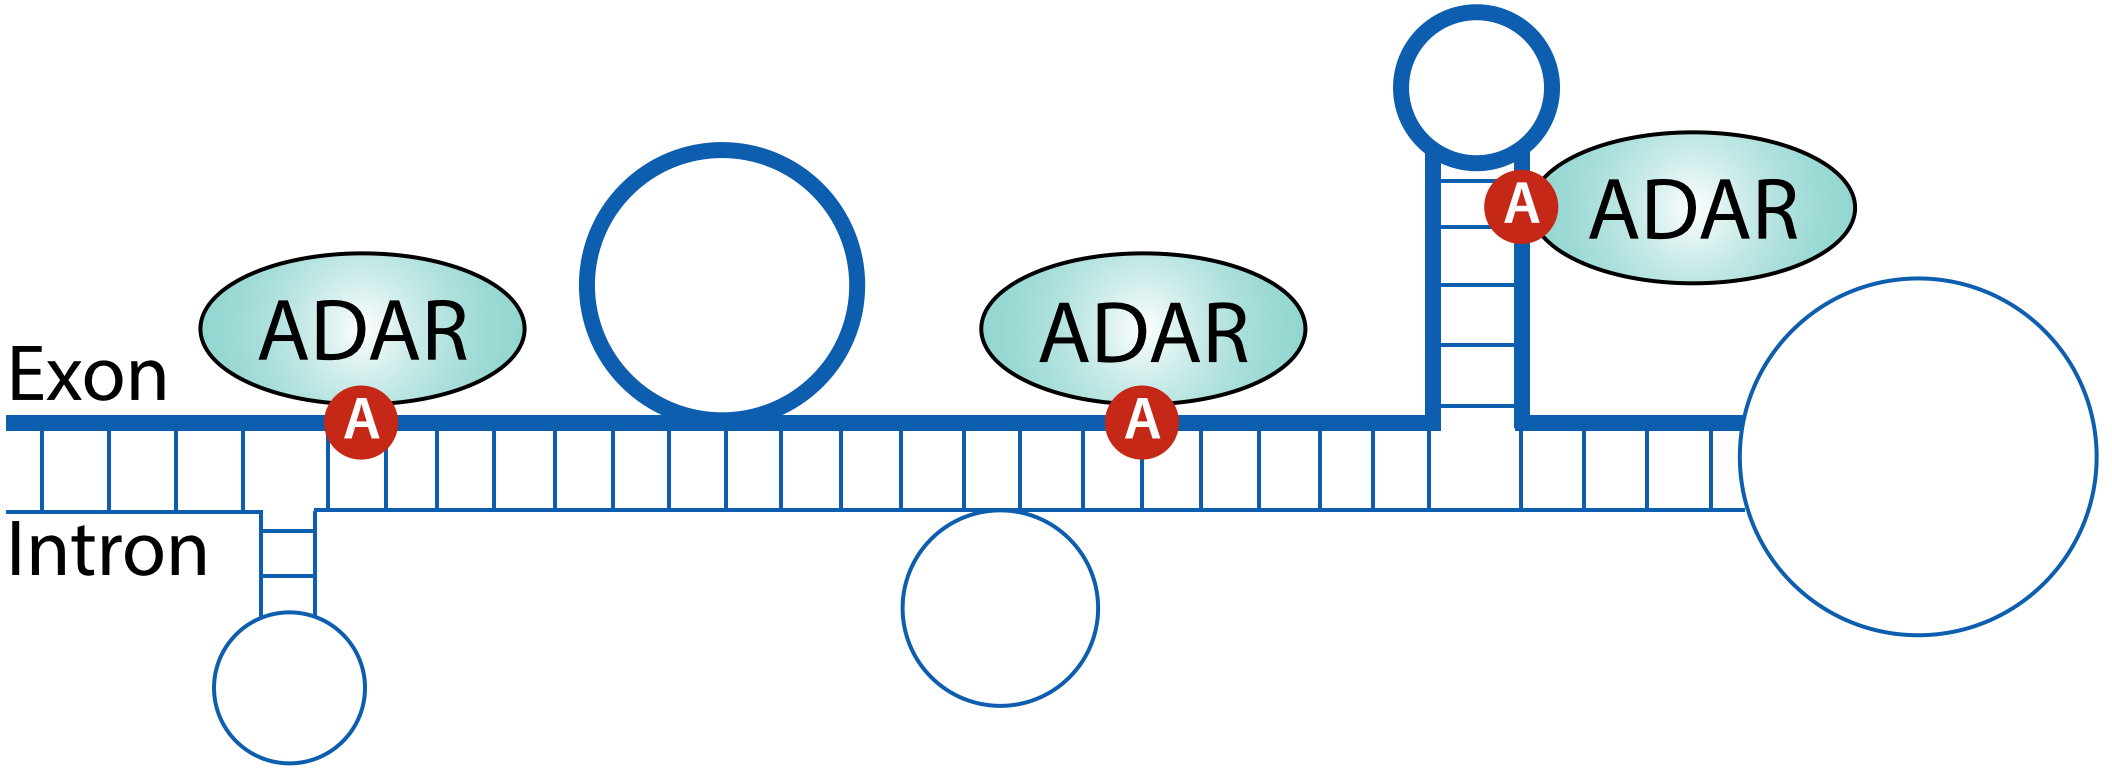
\includegraphics[width=14cm]{ADAR.png}
	\end{center}
	\caption{ADARの作用機序}
	\begin{flushleft}
		\normalsize{ADARは二次構造を形成した二本鎖RNAへ結合し、A-to-I editingを触媒する。多くの転写物は一つ以上の複数のeditingサイトを持つ。}
	\end{flushleft}
\end{figure}

\subsection{ADARのドメイン構造}
ADARはA-to-I editingを触媒するdeaminaseドメインと二本鎖RNAに結合するdsRBD (Double-strand binding domain)の2つを共通して有している。dsRBDは65残基程度の長さの中にα-β-β-β-αという特徴的なドメイン構造を持ち、直接的に二本鎖RNAと接触するためA-to-I editingに必須の機能ドメインの一つである。ADAR1においては、Z-DNA-bindingドメインを2つ有しているが、機能的な意味については不明である。ADAR3のみに特徴的にアルギニンリッチな一本鎖RNA結合ドメインのR-domainを持つ。

\begin{figure}[htbp]
	\begin{center}
		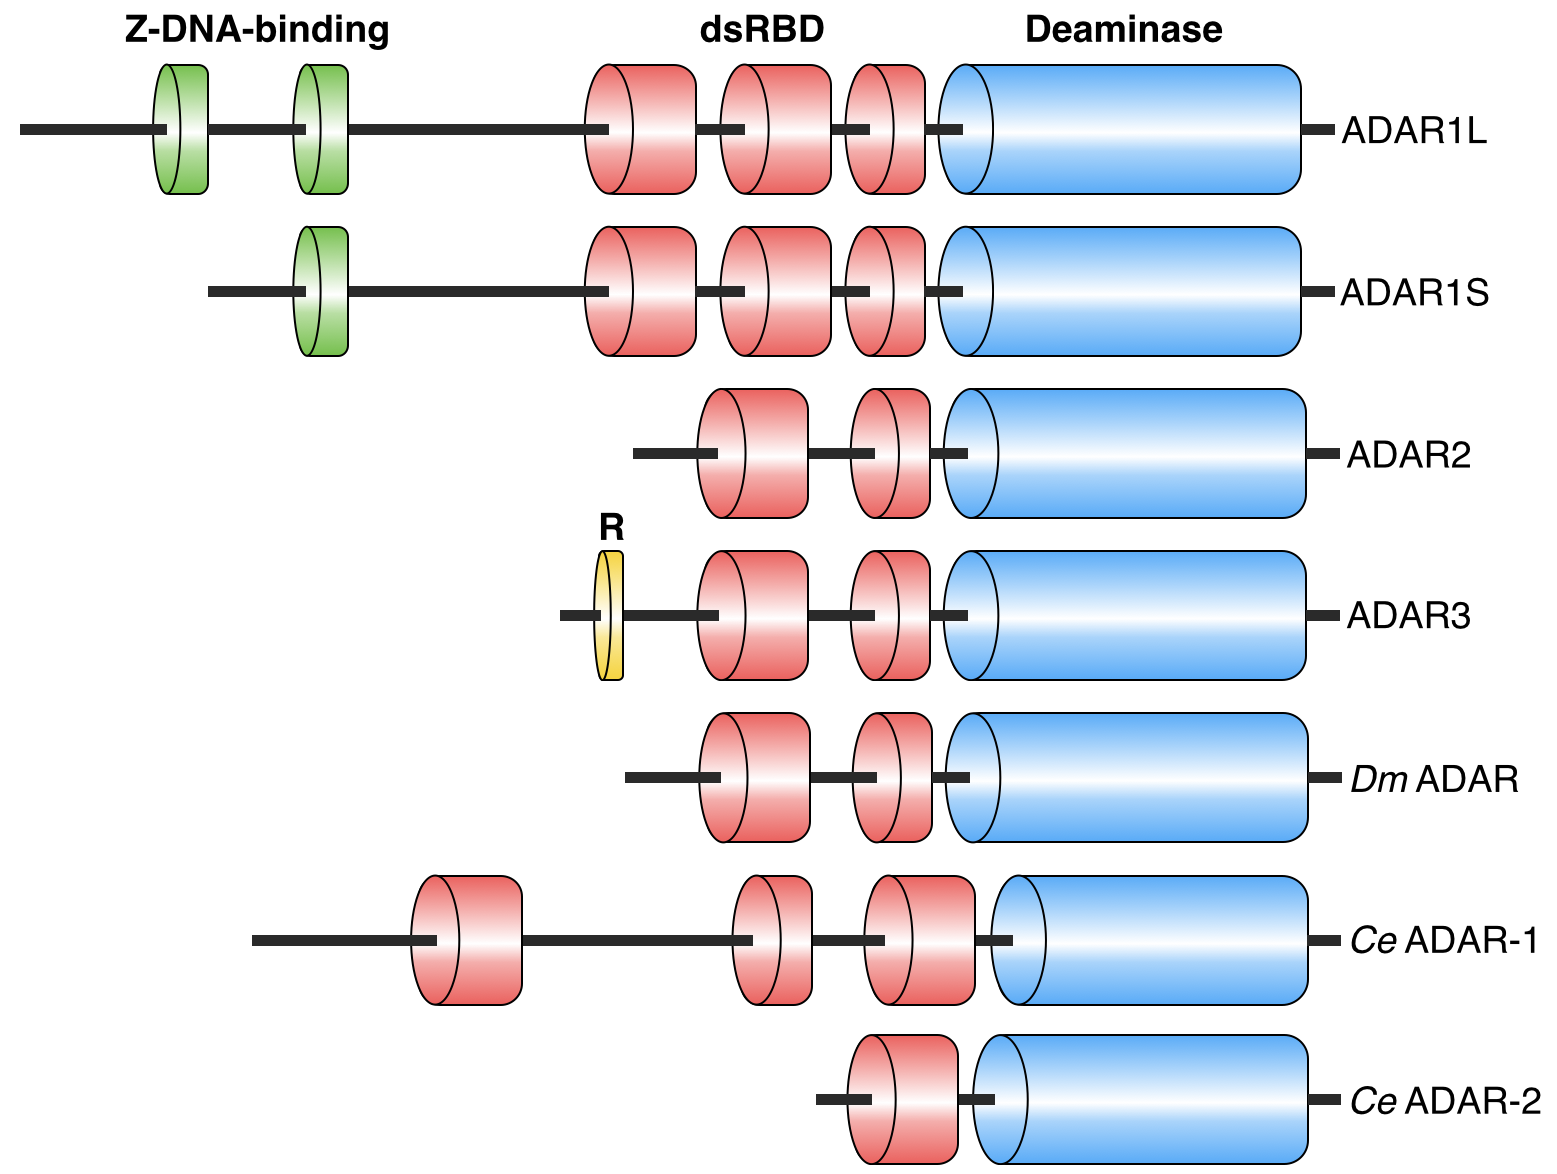
\includegraphics[width=14cm]{Adar_domain.png}
	\end{center}
	\caption{ADARのドメイン構造}
\end{figure}

\subsection{ADARの発現と細胞内局在}
ヒトにおいては、これまでにADAR1、ADAR2、ADAR3の3種類が同定されており、そのうちADAR1については核内および細胞質に局在するADAR1LおよびADAR1Sが知られる他、ADAR3は脳特異的に発現することが知られている。ヒトにおけるADAR1およびADA2は、上記2つの機能ドメインの他にもZ-DNA結合ドメインを有している。
マウス、ショウジョウバエ、線虫におけるADARはバリアントが複数同定されている。

\section{遺伝子領域におけるA-to-I editing}
\subsection{タンパク機能の多様化}

\section{非コード領域におけるA-to-I editing}
\subsection{反復配列におけるA-to-I editing}

\subsection{miRNAへのeditingと遺伝子発現制御}
\subsection{A-to-I editingとRNAiのクロストーク}
\subsection{A-to-I editingとスプライシングの関係性}

\section{情報学的解析によるRNA editingサイトの検出}
\subsection{超並列シーケンサーによる網羅的解析}
ここ数年、超並列シーケンサーに代表される配列決定技術の躍進的な発展は、多サンプルのゲノムおよびトランスクリプトームのシーケンスを可能にしてきた。RNA editing研究においては、超並列シーケンサーから得られるRNA-seqデータやDNA-seqデータを用いることにより、網羅的で定量性のあるeditingサイトを検出する情報学的手法が精力的に開発されている。超並列シーケンサーから測定されるトランスクリプトームやゲノムの配列情報は、数GBから数百GBの配列データを扱うことになるため、editingサイトの検出は本質的に情報学的な解析が必須となっている。2009年にLiらは、初めてヒトB細胞のRNA-seqデータを用いることにより、10,000箇所を超えるeditingサイトがゲノムワイドに同定されたと報告した。検出された修飾のパタンは、ADARによるA-to-I editing以外にも、A-to-T editingなど未知の修飾の可能性が残されていることを示唆する議論を展開した。また、同定されたeditingサイトは遺伝子間領域にも豊富に分布していること、アミノ酸置換を伴うeditingサイトを新規に同定したと報告した。ところが、この研究が掲載された後、3つの解析結果に対する追従論文が発表され、Liらによる解析結果の95\%以上は擬陽性の可能性があること、解析における擬陽性の原因と排除するための統計的な手法についての提案がされた。

こういったRNA-seqデータを用いることによるゲノムワイドなeditingサイトの分布が明らかになるにつれて、ヒトやマウス、ショウジョウバエといった高等真核生物におけるRNA editingの作用機序、生体内における機能そのものを大きく拡張することになった。
タンパク質の触媒部位へ作用することにより、

\subsection{検出手法の開発}
\subsection{組織およびセルライン特異的なRNA editing}
